%%%%%%%%%%%%%%%%%%%%%%%%%%%%%%%%%%%%%%%%%%%%%%%%%%%%%%%%%
\chapter[Présentation d’eLua]{Présentation d’eLua}
\label{chap:chap3}

\section{Qu'est-ce que Lua?}

Lua est un langage de script libre, réflexif et impératif. Il a été conçu afin de pouvoir être embarqué au sein d'autres applications et les étendre
Lua (qui signifie lune en portugais) a été développé par des membres du groupe de recherche TeCGraf, de l'université de Rio de Janeiro au Brésil.
Il est écrit en langage C ANSI strict, et grâce a cela il est compilable sur une grande variété de systèmes; le plus souvent est utilisé dans des systèmes 
embarqués, dont sa compacité est très appréciée, de plus, il possède la compatibilité du langage Cpour s'intégrer facilement dans la plupart des projets.
Il profite de la compatibilité que possède le langage C avec un grand nombre de langages pour s'intégrer facilement dans la plupart des projets. Lua a déjà
été utilisé pour le développement de jeux vidéo, entre eux, par exemple l'interface du jeu World of Warcraft de Blizzard Entertainment, SimCity4, entre 
autres.

\begin{figure}[h]
\begin{center}

\includegraphics[scale=1]{figure/eLua/Lua.JPG}
\caption{Logo Lua}
\end{center}
\end{figure}


\section{Qu'est-ce qu'eLua?}

  elua adopte le langage de programmation Lua pour faire une complète implémentation dans le monde de l'embarqué, elua ajoute des caractéristiques
spécifiques pour une efficacité, portabilité et développement de logiciels embarqués. eLua propose la totalité des caractéristiques de la version
de bureau de Lua, et c'est important de remarqué que elua utilise les mécanismes de base pour pouvoir l'étendre avec des fonctionnalités de développement 
de l'embarqué optimisés et spécifiques.
 

\subsection{Architecture de eLua}

\begin{figure}[h]
\label{elua}
\begin{center}
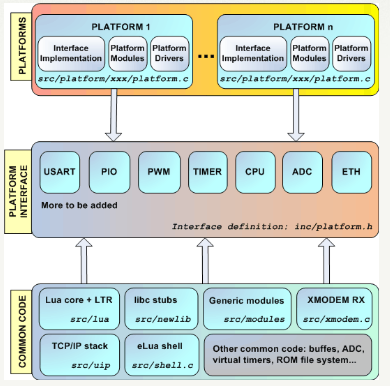
\includegraphics[scale=0.6]{figure/eLua/schema.png}
\caption{Structure logique de eLua}

\end{center}
\end{figure}

  Dans la documentation de eLua on utilise la notion de ``plateforme'' pour designer un groupe de CPU qui partagent la même structure du noyau; pourtant
ils peuvent différer dans le nombre de péripheriques integrés, la mémoire interne, et toute autres attributs. Un port eLua implemente un ou plusieurs
CPU d'une même plateforme.
Dans la figure~\ref{elua}, on observe que eLua essaie d'être aussi portable que possible dans différents plateformes, pour cela plusieurs règles ont été mises en
place, entre elles:

\begin{itemize}
 \item Le code qui est indépendant du type de plateforme doit être écrit en ANSI C dans toutes les parties ou cela est possible, afin qu'il soit
portable parmi plusieurs architectures et compilateurs, comme Lua. 

 \item Le code qui ne peut pas être générique (par exemple le péripheriques et le code spécifique au CPU) doit être fait aussi portable que possible en
utilisant une interface en commun qui doit être implementé par toutes les plateformes dans lequelles eLua peut être executé. On va l'appeler ``interface
de plateforme'' (à complèter avec la documentation).

 \item Toutes les plateformes et leur péripheriques ne sont pas crées de la même façon et possèdent donc des fonctionnalités très variés. Pour accèder
a une fonctionnalité spécifique à une plateforme on peut utiliser un module (voir dans la documentation). Ces modules ont été crées afin de complèter 
l'écart entre l'interface de la plateforme et toutes les caractéristiques proposés par la plateforme.
toutes les fonct
  
\end{itemize}

\subsection{Code en commun}

La liste suivante montre quelques éléments qui sont classifiés comme du code en commun:

\begin{itemize}
 \item Le code Lua
 \item Tous les composants eLua (par exemple le ROM file system, le shell eLua, et autres)
 \item Tous les modules génériques, qui sont des modules exportés de Lua
 \item Le code générique des péripheriques
\end{itemize}

C'est important de remarquer que les parties génériques doivent être la plupart du code. Par exemple, lorsqu'on veut ajouter un nouveau fichier du système
celui-ci doit être un code générique, sinon le code aura des dependances par rapport où il reside. On peut corriger cela en utilisant des fonctions
définies dans l'interface de la plateforme, mais si cela n'est pas possible il faudra séparer les fonctions spécifiques dans une interface separé qui va
devoir être implementé par toutes les plateformes qui veulent utiliser ce nouveau fichier. Ceci donne un maximum de portabilité au code.

L'utilisateur ne doit jamais oublier le but principal de eLua: la flexibilité. Il doit donc être dans la capacité de savoir quelles composants font partie
de son binaire eLua, de même pour les modules, il doit savoir quels modules il a besoin.
L'utilisateur est demandé de faire leur code pour différents scénarios possible, afin de promouvoir la portabilité.

\section{Avantages de eLua}

\begin{description}

 \item[Contrôle total de la plateforme:] il n'existe pas un systèmee d'exploitation entre les programmes et le microcontrôleur.
 
 \item[Portabilité du code:] Comme Lua, le programme peut être executée dans un grand groupe varié de plateformes et architectures.

 \item[Facilité de transformation:] Le code et le design des produits pour eLua peuvent être conçu indépendament du matériel, ainsi toute changement ou
amélioration dans le future peut être fait facilement et gagner du temps.

 \item[Développement d'objectifs:] Lua est complètement fonctionnel avec la possibilité d'avoir un shell dans le microcontrôleur, il n'y a pas besoin 
de rien installer côté ordinateur a part la connexion du port ou ethernet. Les programmes sont utilisable directement dans les plateformes.

 \item[Flexibilité des produits:] L'utilisation de ce langage script de très haut niveau dans un projet rend celui-ci très adaptable, facilement
reprogrammable et reconfigurable. Les systèmes sont très efficients pour une future évolution.

 \item[Embarqué RAD:] Prototype et experimenté dans un modèle ``Rapid Aplication Develop''. Les idées peuvent être testé directement dans les plateformes
avec les kits de développement; l'utilisateur n'a pas besoin des simulateurs ou des futures modification du code pour le rendre adaptable.

 \item[Les kits sont prêts a être utilisés :] Grand nombre des logiciels open source et plateformes sont utilisables.

 \item[Long cycle de vie:]  Add user configuration and scripting capabilities to your projects, making them adaptable to the always changing contexts of industrial processes, evolving engineering, automation standards, field optimizations etc...

 \item[Apprendre l'embarqué: ] L'experimentation est très simple et interactive. L'utilisateur est invité a utiliser ses compètences en programmation
pour devenir un développeur des systèmes embarqués rapidement et de façon amusante.

 \item[Open Source:] elua est libre, gratuit, et open source logiciel, comme Lua, elle possède une licence MIT qui permet l'utilisation de eLua dans des 
codes ``closed'' source. Il n'y a aucune permission a demander, ils demandent juste de faire circuler l'information au monde: on utilise eLua!
\end{description}




